\documentclass[tikz,border=10pt]{standalone}
\usepackage{tikz}
\usepackage{amsmath}

\begin{document}
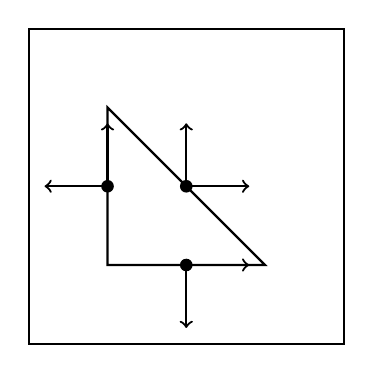
\begin{tikzpicture}[scale=2]
    % Define the vertices of the reference triangle

    \coordinate (G0) at (-0.5,-0.5);  
    \coordinate (G1) at (-0.5,1.5);  
    \coordinate (G2) at (1.5,1.5);  
    \coordinate (G3) at (1.5,-0.5);  
    \draw[black, thick] (G0) -- (G1) -- (G2) -- (G3) -- cycle;



    \coordinate (A) at (0,0);
    \coordinate (B) at (1,0);
    \coordinate (C) at (0,1);
    \coordinate (N1) at (0.5,0);
    \coordinate (N2) at (0,0.5);
    \coordinate (N3) at (0.5,0.5);

    \draw[black, thick] (A) -- (B) -- (C) -- cycle;

    \draw[->, black, thick] (0.5, 0) -- (0.5, -0.4);   
    \draw[->, black, thick] (0.5, 0) -- (0.9, 0);   
    \draw[->, black, thick] (0.5, 0.5) -- (0.5,0.9);   
    \draw[->, black,  thick] (0.5, 0.5) -- (0.9,0.5);   
    \draw[->, black, thick] (0, 0.5) -- (-0.4, 0.5);  
    \draw[->, black, thick] (0, 0.5) -- (0.0, 0.9);  

    \fill[black] (N1) circle (0.04);
    \fill[black] (N2) circle (0.04);
    \fill[black] (N3) circle (0.04);

\end{tikzpicture}
\end{document}



